\documentclass[a4paper,12pt]{book}

% PACKAGES DE BASE
\usepackage[english,french]{babel}
\usepackage[utf8]{inputenc}
\usepackage[T1]{fontenc}

% PACKAGES ADDITIONNELS
\usepackage{color}  % pour utiliser des couleurs
\usepackage{enumitem} % pour personnaliser les puces
\usepackage{fancyhdr}  % Personnalisation en-tête et pied de page
\usepackage[top=2.5cm, bottom=2.5cm, left=2.8cm, right=2.8cm]{geometry} % Pour redimensionner les marges
\usepackage{graphicx}  % Pour l'insertion d'images
\usepackage[hyphens]{url}  % Pour insérer des url. l'option 'hyphens' permet de ne pas afficher de barre oblique au niveau de la césure d'une url.
\usepackage{listings}  % Pour définir un environnement de citation de code
\usepackage{tcolorbox}  % Pour le paramètrages des box
\usepackage{titlesec}  % Pour personnaliser les titres des chapitres
\usepackage{verbatim}  % pour les citations de code
\usepackage{xcolor}  % pour utiliser des couleurs
% Package à supprimer
\usepackage{lipsum}
% Package à placer en dernier
\usepackage{hyperref}

% PARAMETRAGE DES URL FIGURANT DANS LE DOCUMENT PDF
\hypersetup{
    colorlinks=true, % Couleur les liens au lieu de les encadrer
    linkcolor=link_table_of_contents,  % Couleur des liens internes (table des matières, références, etc.)
    urlcolor=pythonblue,   % Couleur des liens URL
}

% DEFINITION DES COULEURS
\definecolor{backcolour}{rgb}{0.95,0.95,0.92}
\definecolor{codegreen}{rgb}{0,0.6,0}
\definecolor{pythonblue}{RGB}{54,117,171}
\definecolor{pythonyellow}{RGB}{220,176,30}
\definecolor{graylight}{RGB}{231,231,231}
\definecolor{link_table_of_contents}{RGB}{65,0,0}

% PERSONNALISER LES TITRES DES CHAPITRES
\titleformat{\chapter}[frame]
  {\normalfont\Huge\bfseries\color{pythonblue}}
  {\textcolor{pythonyellow}{Challenge N°}\ \textcolor{pythonyellow}{\thechapter}}
  {25pt}
  {\Huge\centering}
  

% PERSONNALISER LES TITRES DES SECTIONS
\titleformat{\section}
  {\normalfont\LARGE\bfseries\color{pythonblue}}
  {\textcolor{pythonyellow}{\thesection}}{1em}{}
  {\LARGE} 
 
% CREATION DE COMMANDES
\newcommand{\bigger}{\fontsize{80}{100}\selectfont}  % Police de grande taille

% ENVIRONNEMENT POUR DU CODE PYTHON:
\lstset{
    language=Python,
    aboveskip=5mm,  % Marge avant l'insertion du code
    belowskip=5mm,  % Marge après l'insertion du code
    backgroundcolor=\color{backcolour},
    keywordstyle=\color{purple}, % Couleur mots clés
    commentstyle=\color{olive}, % Coleur commentaires  
    stringstyle=\color{codegreen},  % Style des strings
    basicstyle=\small, % Taille police
    basicstyle=\ttfamily, % Style police
    numbers=left, % Numéros de ligne à gauche
    numberstyle=\scriptsize, % Taille numéros de ligne 
    numbersep=10pt, % Espace entre numéro de ligne et code
    showspaces=false,  % Voir les espaces             
    showstringspaces=false,  % Voir les espaces des strings
    showtabs=false,  % Voir les tabulations               
    tabsize=4,  % Tabulations
    frame=tb,  % Cadre en haut et en bas
    rulecolor=\color{pythonblue},  % Couleur du cadre 
    captionpos=b,  % Position de la légende du code
    morekeywords={assert, randint, insert, pop},
    emph = {colorsys, get_color_types, get_complementary, hls_to_rgb,    	rgb_to_hls, pytest},
    emphstyle=\color{blue},
    literate= % Pour une gestion de l'utf8
        {â}{{\^a}}1 {à}{{\`a}}1 {ç}{{\c c}}1 {é}{{\'e}}1
        {è}{{\`e}}1 {ê}{{\^e}}1 {î}{{\^i}}1 {ô}{{\^o}}1
        {É}{{\`E}}1
        {Ò}{{\`O}}1
        {°}{{\textdegree}}1
}

%%% TEXTE %%%

\begin{document}

% PAGE DE COUVERTURE
\thispagestyle{empty} % Supprime la numérotation de la première page
\begin{center}
\begin{tcolorbox}[colback=graylight, boxrule=2pt, sharp corners, toprule=2pt, bottomrule=2pt] %[frame=double, colback=#f2f2f2]
\begin{minipage}{\textwidth}
    \centering
    \vspace{1.8cm}
    \bigger \textbf{\textcolor{pythonblue}{Challenges Python}} \\
    \vspace{1cm}
    \Large \textbf{\textcolor{pythonyellow}{(Discord \og Docstring\fg{})}}
    
    \vspace{3cm}
    
\includegraphics[width=13cm]{IMG/logo_python.jpeg} 
    
    \vspace{6cm}
    
    \Large \textbf{\textcolor{pythonblue}{@bucdany}} \\
    \vspace{2cm}
    2023
    \vspace{1.2cm}
\end{minipage}
\end{tcolorbox}
\end{center}

% PREMIERE  (vide - première page numérotée)
\clearpage 
\setcounter{page}{1}
\pagestyle{plain}

% TABLE DES MATIERES
\tableofcontents

% DEBUT TEXTE
\chapter*{Avant propos}
\lipsum[1-3]

% CHAPITRE 1
\chapter{Compter le nombre de voyelles}
\vspace{2cm}
\section{Énoncé}
\medskip

Ce premier challenge est très simple, il est de niveau \og débutant\fg{}, mais si vous avez plus d'expérience, vous pouvez essayer de trouver de belles astuces pour un code propre, rapide et concis.
\medskip

Ici, il va nous falloir créer une fonction \verb|nb_voyelles(phrase: str)->int| qui retourne le résultat du nombre total de voyelles dans une phrase passée en paramètre.
\medskip

\subsection*{Conditions}
\begin{itemize}
	\item[-] Les voyelles sont : \texttt{aeiou}, \texttt{y} n’est pas pris en compte.
	\item[-] Les voyelles accentuées ne sont pas prises en compte.
	\item[-] La phrase passée en paramètre doit être écrite en minuscule.
	\item[-] Une chaîne vide, passée en paramètre, doit renvoyer \texttt{0}.
\end{itemize}
\medskip

\subsection*{Exemples}
\begin{itemize}
	\item[\textbullet] \verb|nb_voyelles("bonjour, comment allez-vous ?")| doit retourner \texttt{9}.
	\item[\textbullet] \verb|nb_voyelles("je vais à paris")| doit retourner \texttt{5}.
	\item[\textbullet] \verb|nb_voyelles("docstring")| doit retournet \texttt{2}.
	\item[\textbullet] \verb|nb_voyelles("")| doit retourner \texttt{0}.
\end{itemize}
\medskip

\section{Solution et explications}
\medskip

Voici donc ma solution\footnote{Fil de discussion de ce challenge: \url{https://discord.com/channels/396825382009044994/1142617945139335189}} :
\begin{lstlisting}
def nb_voyelles(phrase: str)->int:
	return sum(phrase.count(el) for el in "aeiou")
\end{lstlisting}
\medskip

\begin{itemize}
	\item[\textbullet] La phrase doit toujours être en minuscule, donc pas besoin de la méthode \texttt{lower()}.
	\item[\textbullet] Ici, on compte chaque voyelle dans la phrase à l'aide de la méthode \texttt{count}.
	\item[\textbullet] La fonction \texttt{sum()} renvoie ensuite la somme du résultat obtenu.
	\item[\textbullet] Si l'on passe un générateur ou une liste de compréhension dans la fonction \texttt{sum()}, la paire de crochets supplémentaire peut-être éliminée\footnote{ Attention, car cela n'est par contre pas compatible avec la fonction \texttt{len()}. Pour plus d'information on se reportera au \texttt{PEP-289}: \url{https://peps.python.org/pep-0289/\#the-details}.}. De cette manière :
	\begin{verbatim}
	sum([phrase.count(el) for el in "aeiou"])
	\end{verbatim}
	est l'équivalent de :
	\begin{verbatim}
	sum(phrase.count(el) for el in "aeiou")
	\end{verbatim}
\end{itemize}
\medskip

Voici aussi le code pour mes tests unitaires :
\begin{lstlisting}
import pytest

@pytest.mark.parametrize("sentence, expected", [
    ("", 0),
    ("docstring", 2),
    ("bonjour comment allez-vous ?", 9),
    ("je vais à paris", 5),
    ("vas-y !", 1),
]) 
def test_should_return_the_sum(sentence, expected):
    got = nb_voyelles(sentence)
    assert got == expected
\end{lstlisting}
\medskip

\texttt{@OsKaR31415} a par ailleurs apporté plusieurs solutions pour résoudre ce challenge\footnote{\url{https://discord.com/channels/396825382009044994/1142617945139335189/1144591818516860998}}.
\chapter{Jeu du \og Pierre - Papier - Ciseaux\fg{}}
\vspace{2cm}
\section{Énoncé}
\medskip

On va jouer un peu en développant un petit jeu très simple.
\medskip

Le but du challenge est de développer le célèbre jeu \og \textit{pierre - papier - ciseaux}\fg{}\footnote{\url{https://fr.wikipedia.org/wiki/Pierre-papier-ciseaux}} en essayant de trouver un algorithme astucieux et un code à la fois simple, propre et efficace.
\medskip

\subsection*{Étapes}
\begin{enumerate}
	\item Générer un choix aléatoire pour votre session de jeu : \og pierre\fg{}, \og papier\fg{} ou \og ciseaux\fg{}.
	\item Demander au joueur d'écrire son choix entre trois propositions : \og pierre\fg{}, \og papier\fg{} ou \og ciseaux\fg{}.
	\item Afficher qui a gagné en dévoilant le choix aléatoire du point n°1.
\end{enumerate}
\medskip

\subsubsection*{Conditions}
\begin{itemize}
	\item[-] L'affichage, le prompt et la réponse seront affichées par écrit sur  la console.
	\item[-] Le fonctionnement du jeu est simple : la pierre gagne sur les ciseaux, les ciseaux gagnent sur le papier, le papier gagne sur la pierre, deux éléments identiques correspondent à une égalité.
	\item[-] Toutes les chaînes de caractères, \og pierre\fg{}, \og papier\fg{} et \og ciseaux\fg{} doivent toujours être entrées en minuscule, le joueur devra donc écrire correctement ces mots, sinon vous devrez lui demander de redéfinir son choix.
	\item[-] S'il y a égalité, vous devrez relancer automatiquement votre programme (en regénérant un nouveau choix aléatoire pour la nouvelle session de jeu), jusqu'à ce qu'il y ait un gagnant à la partie.
\end{itemize}
\medskip

\subsection*{Exemples}
\begin{itemize}
	\item[-] Le choix aléatoire donne \og pierre\fg{} et le joueur a choisi \og papier\fg{} -> \texttt{Vous avez gagné ! Le papier enveloppe la pierre}
	\item[-] Le choix aléatoire donne \og ciseaux\fg{} et le joueur a choisi \og papier\fg{} -> \texttt{Vous avez perdu ! Les ciseaux coupent le papier}
	\item[-] Le choix aléatoire donne \og pierre\fg{} et le joueur a choisi \og pierre\fg{} -> \texttt{Égalité ! Recommencez...}
\end{itemize}
\medskip

\section{Ma solution}
\begin{lstlisting}
from random import randint

BDD = {
    "element": ["papier", "pierre", "ciseaux"],
    "gagnant": ["10", "21", "02"],
    "phrase": ["Le papier enveloppe la pierre",
               "Les ciseaux coupent le papier",
               "La pierre casse les ciseaux"]
}

while True:
    joueur = input("pierre, papier ou ciseaux: ")
    if joueur in BDD["element"]:
        choix, joueur = (randint(0, 2),
                         BDD["element"].index(joueur))

        if choix != joueur: break
        print("Égalité, recommencez...")

    else: print("Faute de frappe !")

print(f'Vous avez {"gagné" if f"{choix}{joueur}" in BDD["g
agnant"] else "perdu"} ! {BDD["phrase"][choix + joueur - 1]
} !')
\end{lstlisting}
\medskip

\section{Explication de l'algorithme}
\subsection*{Contexte}
\begin{itemize}
	\item[-] Trois éléments : \og pierre\fg{}, \og papier\fg{} ou \og ciseaux\fg{}.
	\item[-] Un choix aléatoire fait par la machine et un joueur qui entre son choix au clavier.
\end{itemize}
\medskip

Il suffit donc de réfléchir à un algorithme sympathique pour présenter le code de manière élégante et éviter bien sûr les répétitions.
\medskip

\subsection*{Rangement des données}
Chaque élément est rangé dans cet ordre particulier dans la liste, afin de les faire correspondre en triade logique.
\begin{itemize}
	\item[\textbullet] papier = index(0)
	\item[\textbullet] pierre = index(1)
	\item[\textbullet] ciseaux = index(2)
\end{itemize}
\medskip

\subsection*{Algorithme pour un choix triangulaire}
Si on fait l'addition \texttt{0+1}, on obtient \texttt{1}, alors le jeu se fait entre \og papier\fg{} et \og pierre\fg{}. On cherche ensuite la phrase dans \texttt{phrase} en faisant juste un calcul grâce à la somme \texttt{-1} des deux éléments. Donc en index:  \texttt{1-0 = 0}, et on trouve donc la chaîne de caractères \texttt{"Le papier enveloppe la pierre"}.
\medskip

Si on fait l'addition \texttt{1+2}, on obtient \texttt{3}, alors le jeu se fait entre la \og pierre\fg{} et les \og ciseaux\fg{}. Donc en index, on obtient \texttt{3-1}, soit \texttt{2}. On trouve donc la chaîne de caractères \texttt{"La pierre casse les ciseaux"}.
\medskip

De la même façon, si on fait l'addition \texttt{2+0}, on obtient \texttt{2} et le jeu se fait entre les \og ciseaux\fg{} et le \og papier\fg{}. En index cela donne \texttt{2-1}, soit \texttt{1}, et on tombe sur la chaîne de caractères \texttt{"Les ciseaux coupent le papier"}.
\medskip

\subsection*{\textit{The Winner is...}}
Pour connaître qui gagne, il suffit de convertir en \textit{string} et de joindre les deux caractères d'index du choix et du joueur. Ainsi, \texttt{10} dans \texttt{gagnant} veut dire que le choix aléatoire donne la \og pierre\fg{} (index \texttt{1}) et que le joueur a saisi le \og papier\fg{} (index \texttt{0}). La \og pierre\fg{} contre le \og papier\fg{} fait donc gagner le joueur.
\medskip

On affiche ainsi \texttt{"gagné"} puis la phrase qui suit s'obtient grâce à l'index de la liste \texttt{phrase} de la \texttt{BDD}, calculée par l'addition des deux index: \texttt{1+(0-1)}, ce qui nous donne \texttt{0}, ce qui correspond à la chaîne de caractères \texttt{"Le papier enveloppe la pierre"}.
\medskip

De la même façon pour \texttt{21} et \texttt{02}, cela représente la combinatoire complète des choix gagnants pour le joueur par rapport au choix aléatoire.
\medskip

\subsection*{Conclusion}
On utilise le calcul de la somme \texttt{-1} qui renvoie un objet de type \texttt{int} et qui pemret l'association des deux chaînes de caractères (\textit{string}) pour connaître le gagnant.
\chapter{Couleur complémentaire}
\vspace{2cm}
\section{Énoncé}
Pour ce challenge j’ai choisi un niveau intermédiaire. Les débutants pourront cependant résoudre la première étape en s’aidant de librairies.
\medskip

Le but de ce challenge est de trouver la \textbf{couleur complémentaire}\footnote{\url{https://fr.wikipedia.org/wiki/Couleur_complémentaire}}
\medskip

\subsection*{Étapes}
\begin{enumerate}
	\item Créer la fonction \verb|get_color_types(color:str)->dict| qui permet de convertir le format \textit{RVB hexadécimal} d’une couleur au format \textit{RVB décimal} et \textit{TSL}\footnote{\url{https://fr.wikipedia.org/wiki/Teinte_saturation_lumière}} (anglais : \textit{\textbf{H}ue\textbf{L}ight\textbf{S}aturation}).
	\begin{description}
		\item[\textbullet{} color : [string]] : la couleur RVB codée en hexadécimal, envoyée en paramètre.
		\item[\textbullet{} dict : [dict]] : contient le résultat de la conversion en différents styles d'écriture, contenant les clés et valeurs suivantes :
		\begin{description}
			\item[hex : [str]] : valeur hexadécimale de la couleur passée en paramètre.
			\item[rvb : [list]] : valeurs de chaque éléments RVB en décimal.
			\item[tsl\_norm : [tuple]] : valeurs de chaque élément TSL (teinte en degrés (360°), saturation et luminosité en pourcentage).
			\item[tsl : [tuple]] : valeurs de chaque élément TSL (teinte, saturation et luminosité au format [0-1], soit de type \texttt{float}).
		\end{description}
	\end{description}
	\medskip
	
	\item Afficher le contenu du dictionnaire retourné par cette fonction.
	\medskip
	
	\item Créer la fonction \verb|get_complementary(color:str)->str| pour trouver la couleur complémentaire et la retourne au format hexadécimal.
\end{enumerate}
\medskip

\subsection*{Conditions}
\begin{itemize}
	\item[-] L'affichage se fera via la console.
	\item[-] Les valeurs hexadécimales sont précédées du symbole \og \texttt{\#}\fg{} et les lettres sont en minuscules.
\end{itemize}
\medskip

\subsection*{Exemples}
\begin{verbatim}
- get_color_types("#19021e") -> {'hex': '#19021e', 'rvb': [25, 2, 30],
                                 'tsl_norm': ('289°', '88%', '6%'), 
                                 'tsl': (0.8035714285714285, 0.875,
                                         0.06274509803921569)}
- get_complementary("#19021e") -> "#071e02"
\end{verbatim}
\medskip

\subsection*{Ressource}
Vous pouvez vous aider du site \texttt{colorpicker}\footnote{\url{https://colorpicker.me/\#00ee7b}} pour vos tests. 
\medskip

\begin{figure}[h]
    \centering
    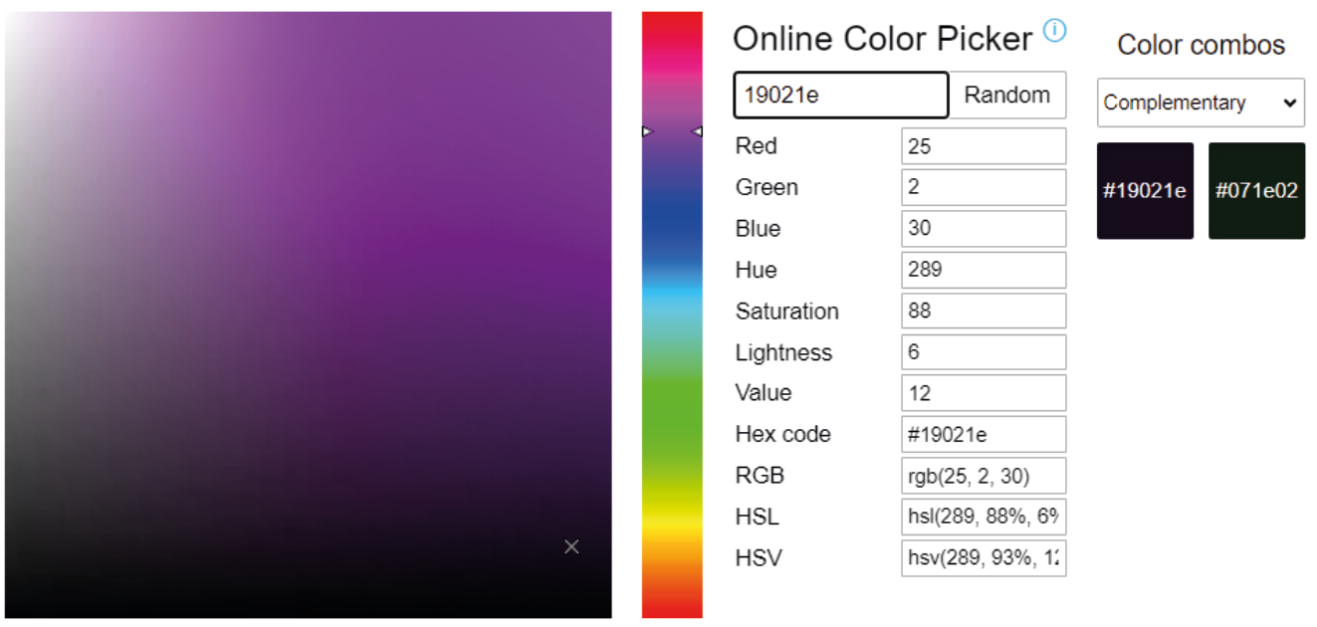
\includegraphics[width=0.8\textwidth]{IMG/color_picker.png}
    \caption{\texttt{colorpicker}}
    \label{fig:colorpicker}
\end{figure}

\subsection*{Indices}
\begin{itemize}
	\item[-] Le nombre hexadécimal d'une couleur représente ses valeurs \textit{RougeVertBleu} codées avec six nombres. Les deux premiers correspondent à la couleur rouge, les deux suivants au vert et les deux derniers au bleu. Pour transformer cette valeur hexadécimale en décimal, il vous suffit de convertir chacune des paires de ce nombre.
	\item[-] Vous pouvez vous aider de la librairie \texttt{colorsys} pour vous permettre de réaliser facilement les conversions.
	\item[-] Ce sont principalement les fonctions \texttt{colorsys.rgb\_to\_hls} et \texttt{colorsys.hls\_to \_rgb} qui pourront être utilisées. 
	\item[-] Pour chercher la complémentaire d’une couleur, il faut passer par le format \textit{TSL} en faisant une rotation de 180° sur la teinte et trouver ainsi la position de la couleur diamétralement opposée.
	\item[-] Pour faire une rotation, il faudra bien sûr penser à normaliser la valeur de la teinte \textit{TSL} qui par défaut est de \texttt{[0, 1]} en \texttt{[0°, 360°]} puis faire la rotation en additionnant avec 180°.
\end{itemize}
\medskip

\begin{figure}[h]
    \centering
    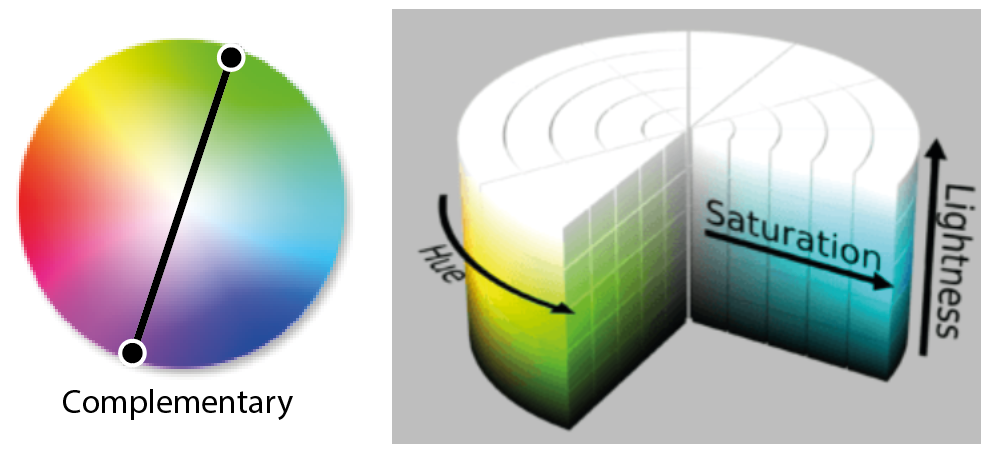
\includegraphics[width=0.8\textwidth]{IMG/schema_colors.png}
    \caption{Couleur complémetaire et TSL}
    \label{fig:colorpicker}
\end{figure}
\medskip

\section{Mon code}
\begin{lstlisting}
from colorsys import rgb_to_hls, hls_to_rgb


def get_color_types(color: str) -> dict:
    rvb = [int(color[i:i+2], 16) for i in
           range(1, len(color), 2)]
    tsl = list(rgb_to_hls(*list(map(lambda x: x/255,
                                    rvb))))
    tsl.insert(-1, tsl.pop())
    tsl_norm = (f"{round(tsl[0]*360)}°",
                *[f"{el:.0%}" for el in tsl[1:3]])
    return {"hex": color, "rvb": rvb,
            "tsl_norm": tsl_norm, "tsl": tuple(tsl)}


def get_complementary(color: str) -> str:
    t, s, l = get_color_types(color)["tsl"]
    return f'#{"".join([f"{round(el*255):02x}" for el 
                        in hls_to_rgb(t+.5 % 1, l, s)])}'
\end{lstlisting}
\medskip

\section{Explications}
\subsection*{Contexte}
Il s'agit soit de faire tous les calculs à la main pour les conversions entre les formats de couleur, soit trouver une bibliothèque qui nous permet de nous simplifier la vie. Mon choix s'est porté sur la bibliothèque \texttt{colorsys} qui est plutôt sympathique pour cela. Elle nous permet de passer au format \texttt{TSL} via \texttt{RGB} et vice et versa.
\medskip

Le but est aussi de trouver la couleur complémentaire, qui est la couleur diamétralement opposée sur le cercle chromatique. Pour cela \texttt{TSL}, nous permet de faire une rotation et trouver directement cette valeur sans difficulté particulière.
\medskip

\subsection*{Différentes problématiques}
\begin{description}
	\item[\textbullet{} Le dièze \og \texttt{\#}\fg{}... gênant hein !] : il y a donc plusieurs façon de faire, soit un simple \texttt{lstrip()} et hop viré, soit débuter son index à \texttt{1}.
	\item[\textbullet{} Conversion d'un format hexadécimal à un format décimal pour le \texttt{RVB}] : \\ un simple \texttt{int(..., 16)} nous fait le calcul directement !
	\item[\textbullet{} Normaliser ses valeurs] : avec la bibliothèque \texttt{colorsys}, attention à toujours rester dans un domaine de valeurs comprises entre \texttt{0} et \texttt{1}, comme stipulé dans la documentation officielle de \texttt{colorsys}\footnote{\url{https://docs.python.org/3/library/colorsys.html} : \og \texttt{the coordinates are all between 0 and 1...}\fg{}}.
	\item[\textbullet{} \texttt{HLS} vs \texttt{TSL}] : attention à bien penser à inverser la saturation de la luminosité si vous utilisez la bibliothèque \texttt{colorsys}.
	\item[\textbullet{} \textit{Tuple}, \textit{liste}] : l'énoncé précise de bien respecter les différents types dans le dictionnaire renvoyé par la fonction.
	\item[\textbullet{} Utilisation des fonctions déjà crées] : on a déjà développé la fonction \texttt{get\_color \\ \_type()} alors pourquoi ne pas l'utiliser pour créer la fonction \texttt{get\_complementar \\ y()} afin d'avoir directement la valeur \texttt{TSL}.
	\item[\textbullet{} Trouver la valeur diamétralement opposée] : une rotation de \texttt{180°} ou de \texttt{0.5} dans la plage de limites [\texttt{0} - \texttt{1}] puis un \textit{modulo} de \texttt{1} à appliquer pour rester dans cette plage de valeurs.
\end{description}
\medskip

\subsection*{Explication du code et astuces d'optimisation / \textit{refactoring}}
\begin{lstlisting}
rvb = [int(color[i:i+2], 16) for i in
           range(1, len(color), 2)]
\end{lstlisting}
\medskip

On pointe avec un \texttt{range} sur la chaîne de caractères \texttt{color} avec un index de \texttt{1} jusqu'à sa taille totale suivant un pas de \texttt{2}, puis avec \texttt{[i:i+2]} on vient chercher deux par deux les caractères hexadécimaux de chaque couleur à convertir en décimal.
\medskip

\begin{lstlisting}
tsl = list(rgb_to_hls(*list(map(lambda x: x/255, rvb))))
\end{lstlisting}
\medskip

Pour constituer notre \texttt{TSL}, on utilise la fonction \texttt{colorsys.rgb\_to\_hls()}. J'ai volontairement utilisé la fonction \texttt{map()} pour vous permettre de voir de nouvelles choses en plus de la compréhension de liste. Ceci \texttt{list(map(lambda x: x/255, rvb))} est la même chose que cela : \texttt{[x/255 for x in rvb]}. C'est juste une autre façon de faire ! Donc on vient diviser chaque couleur \texttt{R}, \texttt{V} et \texttt{B} par \texttt{255} pour respecter la norme \texttt{0} à \texttt{1} qui sera nécessaire pour l'argument de la fonction \texttt{rgb\_to\_hls()}. Notez l'astérisque (\texttt{*}) qui permet de faire un \textit{unpacking} pour dispatcher les éléments \texttt{RVB} en trois arguments, la fonction \texttt{rgb\_to\_hls()} nécessitant trois arguments pour fonctionner. Et l'on convertit en \texttt{list()} car nous avons ensuite besoin d'intervertir les deux derniers éléments, luminosité et saturation étant inversés par rapport à l'énoncé du challenge.
\medskip

\begin{lstlisting}
tsl.insert(-1, tsl.pop())
\end{lstlisting}
\medskip

C'est la phrase magique qui permet d'inverser les places des deux derniers éléments de la liste. \texttt{pop()} permet de retirer le dernier élément, 
\texttt{insert()} permet d'insérer ce que \texttt{pop()} renvoie à l'index \texttt{-1}, qui est l'avant dernière position... \texttt{-1} étant la dernière position mais l'insertion se passe juste avant la position indiquée, donc juste avant \texttt{-1}. La liste \texttt{tsl} sera alors modifiée directement.
\medskip

\begin{lstlisting}
tsl_norm = (f"{round(tsl[0]*360)}°",
                *[f"{el:.0%}" for el in tsl[1:3]])
\end{lstlisting}
\medskip

On utilise le résultat de la conversion \texttt{TSL} pour obtenir \texttt{TSL\_norm}:
\begin{itemize}
	\item[-] La teinte est définie en degrés, comprise dans une limite entre 0 et 360°. \texttt{round()} permet d'arrondir pour avoir une valeur sans chiffre après la virgule. 
	\item[-] La luminosité et la saturation quant à elles sont exprimées en pourcentage grâce à l'utilisation d'une \textit{f-string} qui avec \og \texttt{\%}\fg{} permet à la fois de multiplier par \texttt{100} et d'afficher le pourcentage. Le \texttt{.0} permet de supprimer les chiffres après la virgule. \texttt{tsl[1:3]} c'est la lecture des élément \texttt{1} et \texttt{2} de la liste \texttt{tsl}. On utilise encore l'astérisque (\texttt{*}) pour avoir en tout trois arguments pour \texttt{tsl\_norm}.
\end{itemize}
\medskip

\begin{lstlisting}
return {"hex": color, "rvb": rvb,
            "tsl_norm": tsl_norm, "tsl": tuple(tsl)}
\end{lstlisting}
\medskip

Juste un simple \texttt{return} pour renvoyer un dictionnaire. Notez le \texttt{tuple()} qui permet de convertir notre précédente liste en tuple afin de suivre l'énoncé du challenge.
\medskip

\begin{lstlisting}
t, s, l = get_color_types(color)["tsl"]
\end{lstlisting}
\medskip

On envoie le résultat \textit{TSL} du dictionnaire de la fonction précédente dans les variables \texttt{t}, \texttt{s} et \texttt{l}. Il est important d'utiliser \texttt{tsl} plutôt que \texttt{tsl\_norm} afin de travailler sur des valeurs non arrondies et avoir ainsi plus de précision.
\medskip

\begin{lstlisting}
return f'#{"".join([f"{round(el*255):02x}" for el 
                        in hls_to_rgb(t+.5 % 1, l, s)])}'
\end{lstlisting}
\medskip

Ce \texttt{return} peut paraître un peu complexe mais tout deviendra simple une fois décomposé :
\medskip

\begin{verbatim}
t+.5 % 1
\end{verbatim}
\medskip

On effectue une rotation de la teinte de \texttt{180°} mais comme on se trouve dans un espace compris entre 0 à 1, alors cela devient \texttt{180/360 = 1/2 = 0.5}. Pour rester dans la norme, on fait un \textit{modulo} \texttt{1}.
\medskip

\begin{verbatim}
hls_to_rgb(t+.5 % 1, l, s)
\end{verbatim}
\medskip

On convertit en \textit{RVB} via \textit{TSL}, avec la teinte, la luminosité et la saturation.
\medskip

\begin{verbatim}
[f"{round(el*255):02x}" for el in hls_to_rgb(t+.5 % 1, l, s)]
\end{verbatim}
\medskip

Cette compréhension de liste nous fournit le \textit{RVB} au format hexadécimal. Il faut pour ça changer la norme et passer de \texttt{[0-1]} à \texttt{[0-255]} en multipliant par \texttt{255} puis convertir en hexadécimal via \texttt{02x}, ce qui nous donne deux chiffres (les valeurs de 0 à 9 seront écrites à l'aide de deux chiffres : 01 02 03 04... 09), \texttt{x} permet la conversion grâce à une \textit{f-string}.
\medskip

\begin{verbatim}
f'#{"".join([f"{round(el*255):02x}" for el 
                        in hls_to_rgb(t+.5 % 1, l, s)])}'
\end{verbatim}
\medskip

\texttt{"".join()} permet de réunir le résultat de chaque paire \textit{RVB}/\textit{hexadécimal} et enfin le \og \texttt{\#}\fg{}, la cerise sur le gâteau !
\medskip

\subsection*{Mon fichier d'\textit{unitests}}
\begin{lstlisting}
import pytest

@pytest.mark.parametrize("hexcode, expected", [
    ("#19021e", {'hex': '#19021e', 'rvb': [25, 2, 30],
                 'tsl_norm': ('289°', '88%', '6%'),
                 'tsl': (0.8035714285714285, 0.875,
                         0.06274509803921569)}),
    ("#aedd5f", {'hex': '#aedd5f', 'rvb': [174, 221, 95],
                 'tsl_norm': ('82°', '65%', '62%'),
                 'tsl': (0.22883597883597884,
                         0.6494845360824743,
                         0.6196078431372549)}),
    ("#ff0000", {'hex': '#ff0000', 'rvb': [255, 0, 0],
                 'tsl_norm': ('0°', '100%', '50%'),
                 'tsl': (0.0, 1.0, 0.5)})
])
def test_different_colour_writing_formats(
        hexcode, expected):
    got = get_color_types(hexcode)

    assert got == expected

@pytest.mark.parametrize("hexcode, expected", [
    ("#19021e", "#071e02"),
    ("#aedd5f", "#8e5fdd"),
    ("#ff0000", "#00ffff"),
])
def test_for_complementary_color_in_hex(
        hexcode, expected):
    got = get_complementary(hexcode)
\end{lstlisting}
\medskip

\subsection*{Quelques conseils}
\begin{itemize}
	\item[\textbullet] Faire fonctionner son code le plus tôt possible en évitant les problèmes.
	\item[\textbullet] Coder simplement pour obtenir un premier jet et optimiser/refactoriser par la suite
	\item[\textbullet] Ne pas hésiter pas à s'aider de bibliothèques, mais il est possible de réaliser tous les calculs à la main pour s'entraîner si on le souhaite.
	\item[\textbullet] Le but n'est pas d'obtenir le code le plus court, mais un code lisible et optimisé avec un algorithme efficace. Penser qu'un code n'est pas seulement pour son usage personnel, surtout si on travaille en \textit{open source}, donc veiller a ce qu'il soit clair. Ne pas hésiter à ajouter des commentaires, cela nous servira tout autant quand nous reverrons notre code trois mois plus tard sans y avoir touché !
\end{itemize}
\medskip


\end{document}